% Copyright 2006 by Till Tantau
%
% This file may be distributed and/or modified
%
% 1. under the LaTeX Project Public License and/or
% 2. under the GNU Free Documentation License.
%
% See the file doc/generic/pgf/licenses/LICENSE for more details.


% \section{Tutorial: Euclid's Amber Version of the \emph{Elements}}
\section{教程:Euclid《几何原本》的琥珀版本}

\bohs

% In this third tutorial we have a look at how \tikzname\ can be used to
% draw geometric constructions.
在这第三篇教程中,我们看看如何用 \tikzname\ 实现几何作图。

% Euclid is currently quite busy writing his new book series, whose
% working title is ``Elements'' (Euclid is not quite sure whether this
% title will convey the message of the series to future generations
% correctly, but he intends to change the title before it goes to the
% publisher). Up to know, he wrote down his text and graphics on
% papyrus, but his publisher suddenly insists that he must submit in
% electronic form. Euclid tries to argue with the publisher that 
% electronics will only be discovered thousands of years later, but the
% publisher informs him that the use of papyrus is no longer cutting edge
% technology and Euclid will just have to keep up with modern tools.
Euclid 最近在忙着写一套新书,书名暂定为“几何原本”(Euclid 不是很确定这个书名是否能把主旨传达给后人,但是他打算在交付给出版商之前修改一下书名)。
到目前为止,他用莎草纸写字画图,但是他的出版商突然要求他必须提交电子版。
Euclid 跟出版商争辩道,电子产品要在几千年后才会发明出来,然而出版商告诉他,莎草纸不再是尖端技术了,他必须得跟上现代工具的步伐。

% Slightly disgruntled, Euclid starts converting his papyrus
% entitled ``Book I, Proposition I'' to an amber version.
Euclid 略带不满,准备把他在莎草纸写的东西转到琥珀上,该部分题为“第 I 卷,命题 1”。

\eohs

% \subsection{Book I, Proposition I}
\subsection{卷 I,命题 1}

\bohs

% The drawing on his papyrus looks like this:\footnote{The text is taken
% from the wonderful interactive version of Euclid's Elements by David
% E. Joyce, to be found on his website at Clark University.}
他在莎草纸上的图是这样的:\footnote{该段文本摘自 David E. Joyce 漂亮的交互式欧几里得几何原本,可以在他 Clark 大学的网站上找到。}
\footnote{{\color{blue} 该段文本原文链接:https://mathcs.clarku.edu/\textasciitilde{}djoyce/java/elements/bookI/propI1.html}}
\footnote{{\color{blue} 该段译文部分参考了:欧几里得\ 著,兰纪正、朱恩宽\ 译. 欧几里得·几何原本. 陕西科学技术出版社, 2003. ISBN 9787536903579.}}

\eohs

% Page 40 of Elements-zh
% 作者:  欧几里得 
% 出版社: 陕西科学技术出版社
% 译者: 兰纪正 / 朱恩宽 
% 出版年: 2003-6
% 页数: 673
% 定价: 38.00元
% ISBN: 9787536903579

\bigskip
\noindent
\begin{tikzpicture}[thick,help lines/.style={thin,draw=black!50}]
  \def\A{\textcolor{input}{$A$}}
  \def\B{\textcolor{input}{$B$}}
  \def\C{\textcolor{output}{$C$}}
  \def\D{$D$}
  \def\E{$E$}
  
  \colorlet{input}{blue!80!black}
  \colorlet{output}{red!70!black}
  \colorlet{triangle}{orange}
  
  \coordinate [label=left:\A]
    (A) at ($ (0,0) + .1*(rand,rand) $);
  \coordinate [label=right:\B]
    (B) at ($ (1.25,0.25) + .1*(rand,rand) $);

  \draw [input] (A) -- (B);
  
  \node [name path=D,help lines,draw,label=left:\D] (D) at (A) [circle through=(B)] {};
  \node [name path=E,help lines,draw,label=right:\E] (E) at (B) [circle through=(A)] {};
  
  \path [name intersections={of=D and E,by={[label=above:\C]C}}];

  \draw [output] (A) -- (C);
  \draw [output] (B) -- (C);

  \foreach \point in {A,B,C}
    \fill [black,opacity=.5] (\point) circle (2pt);

  \begin{pgfonlayer}{background}
    \fill[triangle!80] (A) -- (C) -- (B) -- cycle;
  \end{pgfonlayer}
  
  \node [below right,text width=10cm,align=justify] at (4,3)
  {
    \small
    % \textbf{Proposition I}\par
    \textbf{命题 1}\par
    % \emph{To construct an \textcolor{triangle}{equilateral triangle}
      % on a given \textcolor{input}{finite straight line}.}
    \emph{在一条已知\textcolor{input}{有限直线}上作一个\textcolor{triangle}{等边三角形}.}
    \par
    \vskip1em
    % Let \A\B\ be the given \textcolor{input}{finite straight line}. It
    % is required to construct an \textcolor{triangle}{equilateral
    %   triangle} on the \textcolor{input}{straight line}~\A\B. 
    设 \A\B\ 是已知\textcolor{input}{有限直线}.
    要求在\textcolor{input}{直线} \A\B\ 上作一个\textcolor{triangle}{等边三角形}.

    % Describe the circle \B\C\D\ with center~\A\ and radius \A\B. Again
    % describe the circle \A\C\E\ with center~\B\ and radius \B\A. Join the
    % \textcolor{output}{straight lines} \C\A\ and \C\B\ from the
    % point~\C\ at which the circles cut one another to the points~\A\ and~\B.
    以 \A\ 为中心,\A\B\ 为半径作圆 \B\C\D ;再以 \B\ 为中心,\B\A\ 为半径作圆 \A\C\E ;由两圆交点 \C\ 分别连\textcolor{output}{直线}到 \A 、\B ,得 \C\A 、\C\B .

    % Now, since the point~\A\ is the center of the circle \C\D\B,
    % therefore \A\C\ equals \A\B. Again, since the point \B\ is the
    % center of the circle \C\A\E, therefore \B\C\ equals \B\A. But
    % \A\C\ was proved equal to \A\B, therefore each of the straight
    % lines \A\C\ and \B\C\ equals \A\B. And 
    % things which equal the same thing also equal one another,
    % therefore \A\C\ also equals \B\C. Therefore the three straight
    % lines \A\C, \A\B, and \B\C\ equal one another. 
    % Therefore the \textcolor{triangle}{triangle} \A\B\C\ is
    % equilateral, and it has been  constructed on the given finite
    % \textcolor{input}{straight line}~\A\B.
    因为点 \A\ 为圆 \C\D\B\ 的圆心,所以 \A\C\ 等于 \A\B .
    又因为 \B\ 为圆 \C\A\E\ 的圆心,所以 \B\C\ 等于 \B\A .
    然而已经证明了 \A\C\ 等于 \A\B;所以线段 \A\C\ 、\B\C\ 都等于 \A\B .
    而且等于同量的量彼此相等,因此三条线段 \A\C 、\A\B 和 \B\C\ 彼此相等.
    所以\textcolor{triangle}{三角形} \A\B\C\ 是等边的,并且已经在给定的有限\textcolor{input}{直线} \A\B\ 上作出了该三角形.
  };
\end{tikzpicture}
\bigskip

\bohs

% Let us have a look at how Euclid can turn this into \tikzname\ code.
让我们看看,Euclid 怎么把这张图变成 \tikzname\ 代码。

\eohs

% \subsubsection{Setting up the Environment}
\subsubsection{设置环境}

\bohs

% As in the previous tutorials, Euclid needs to load \tikzname, together
% with some libraries. These libraries are |calc|, |intersections|,
% |through|, and |backgrounds|. Depending on which format he uses,
% Euclid would use one of the following in the preamble:
如之前教程所述,Euclid 需要载入 \tikzname\ 以及一些库,这些库包括 \ltz{calc}、\ltz{intersections}、\ltz{through} 和 \ltz{backgrounds}。
根据格式不同,Euclid 要在序言区加上下列语句之一:

\eohs

\begin{codeexample}[code only]
% 对于 LaTeX:
\usepackage{tikz}
\usetikzlibrary{calc,intersections,through,backgrounds}
\end{codeexample}

\begin{codeexample}[code only]
% 对于 plain TeX:
\input tikz.tex
\usetikzlibrary{calc,intersections,through,backgrounds}
\end{codeexample}

\begin{codeexample}[code only]
% 对于 ConTeXt:
\usemodule[tikz]
\usetikzlibrary[calc,intersections,through,backgrounds]
\end{codeexample}


% \subsubsection{The Line \emph{AB}}
\subsubsection{线 \emph{AB}}

\bohs

% The first part of the picture that Euclid wishes to draw is the line
% $AB$. That is easy enough, something like |\draw (0,0) -- (2,1);|
% might do. However, Euclid does not wish to reference the two points
% $A$ and $B$ as $(0,0)$ and $(2,1)$ subsequently. Rather, he wishes to
% just write |A| and |B|. Indeed, the whole point of his book is that
% the points $A$ and $B$ can be arbitrary and all other points (like
% $C$) are constructed in terms of their positions. It would not do
% if Euclid were to write down the coordinates of $C$ explicitly.
图中 Euclid 想最先画的部分是线 $AB$。很简单,\ltz{\\draw (0,0) -- (2,1);} 就能搞定。
但是,Euclid 不想在 $A$ 和 $B$ 后面加上 $(0,0)$ 和 $(2,1)$,他想只写上 \ltz{A} 和 \ltz{B}。
事实上,他的书的主旨是,点 $A$ 和 $B$ 可以是任意的,其他的点(比如 $C$)可以根据它们的位置构造出来,Euclid 不需要直接写出 $C$ 的坐标。

% So, Euclid starts with defining two coordinates using the
% |\coordinate| command:
所以 Euclid 用 \ltz{\\coordinate} 命令定义两个坐标:

\eohs

\begin{codeexample}[]
\begin{tikzpicture}
  \coordinate (A) at (0,0);
  \coordinate (B) at (1.25,0.25);

  \draw[blue] (A) -- (B);
\end{tikzpicture}
\end{codeexample}

\bohs

% That was easy enough. What is missing at this point are the labels for
% the coordinates. Euclid does not want them \emph{on} the points, but
% next to them. He decides to use the |label| option:
非常简单。
这里少了坐标的标签,Euclid 不想标在点\emph{上面},而是在点旁边。
他决定用 \ltz{label} 选项:

\eohs

\begin{codeexample}[]
\begin{tikzpicture}
  \coordinate [label=left:\textcolor{blue}{$A$}]  (A) at (0,0);
  \coordinate [label=right:\textcolor{blue}{$B$}] (B) at (1.25,0.25);

  \draw[blue] (A) -- (B);
\end{tikzpicture}
\end{codeexample}

\bohs

% At this point, Euclid decides that it would be even nicer if the
% points $A$ and $B$ were in some sense ``random.'' Then, neither Euclid
% nor the reader can make the mistake of taking ``anything for granted''
% concerning these position of these points. Euclid is pleased to learn
% that there is a |rand| function in \tikzname\ that does exactly what
% he needs: It produces a number between $-1$ and $1$. Since \tikzname\
% can do a bit of math, Euclid can change the coordinates of the points
% as follows:
Euclid 这时在想,要是点 $A$ 和 $B$ 可以“随机”一点就更好了。
关于这些点的位置,Euclid 和读者都不能犯下“想当然”的错误。
Euclid 很高兴地了解到,\tikzname\ 里有一个 \ltz{rand} 函数可以满足要求:它能生成一个 $-1$ 到 $1$ 之间的数。
既然 \tikzname\ 能做些数学运算,Euclid 就可以把点坐标写成下面这样:

\eohs

\begin{codeexample}[code only]
\coordinate [...] (A) at (0+0.1*rand,0+0.1*rand);
\coordinate [...] (B) at (1.25+0.1*rand,0.25+0.1*rand);
\end{codeexample}

\bohs

% This works fine. However, Euclid is not quite satisfied since he would
% prefer that the ``main coordinates'' $(0,0)$ and $(1.25,0.25)$ are
% ``kept separate'' from the perturbation
% $0.1(\mathit{rand},\mathit{rand})$. This means, he would like to
% specify that coordinate $A$ as ``The point that is at $(0,0)$ plus one
% tenth of the vector  $(\mathit{rand},\mathit{rand})$.''
这个效果不错,但是 Euclid 并不是很满意,因为他想让“主坐标” $(0,0)$ 和 $(1.25,0.25)$ 同扰动 $0.1(\mathit{rand},\mathit{rand})$ “分离开来”。
也就是说,他希望将坐标 $A$ 指定成这样,“点 $(0,0)$ 加上向量 $(\mathit{rand},\mathit{rand})$ 的十分之一”。

% It turns out that the |calc| library allows him to do exactly this
% kind of computation. When this library is loaded, you can use special
% coordinates that start with |($| and end with |$)| rather than just
% |(| and~|)|. Inside these special coordinates you can give a linear
% combination of coordinates. (Note that the dollar signs are only
% intended to signal that a ``computation'' is going on; no mathematical
% typesetting is done.)
实际上,\ltz{calc} 库来能让他做这类运算。载入该库后,你可以用特殊的坐标,始于 \ltz{($} 止于 \ltz{$)},而不只是 \ltz{(} 和 \ltz{)}。
你可以对这些特殊的坐标进行线性组合。(注意到 \ltz{$} 符号只是表示开始“运算”,而不是输入数学公式。)

% The new code for the coordinates is the following:
关于坐标的新代码如下:

\eohs

\begin{codeexample}[code only]
\coordinate [...] (A) at ($ (0,0) + .1*(rand,rand) $);
\coordinate [...] (B) at ($ (1.25,0.25) + .1*(rand,rand) $);
\end{codeexample}

\bohs

% Note that if a coordinate in such a computation has a factor (like
% |.1|), you must place a |*| directly before the opening parenthesis of
% the coordinate. You can nest such computations.
注意,如果在这类计算中,一个坐标包含小数(比如 \ltz{.1}),那么你必须在坐标的左圆括号之前加上 \ltz{*}。
这些运算可以嵌套。

\eohs

% \subsubsection{The Circle Around \emph{A}}
\subsubsection{围绕点 \emph{A} 的圆}

\bohs

% The first tricky construction is the circle around~$A$. We will see
% later how to do this in a very simple manner, but first let us do it
% the ``hard'' way.
第一个棘手的构造是围绕点 $A$ 的圆。
我们之后会介绍一个非常简单的方法,但是首先让我们用“困难的”方式实现它。

% The idea is the following: We draw a circle around the point $A$ whose
% radius is given by the length of the line $AB$. The difficulty lies in
% computing the length of this line.
思路如下:我们画一个围绕点 $A$ 的圆,其半径由线段 $AB$ 的长度决定。
困难在于计算这条线段的长度。

% Two ideas ``nearly'' solve this problem: First, we can write
% |($ (A) - (B) $)| for the vector that is the difference between $A$
% and~$B$. All we need is the length of this vector. Second, given two
% numbers $x$ and $y$, one can write |veclen(|$x$|,|$y$|)| inside a
% mathematical expression. This gives the value $\sqrt{x^2+y^2}$, which
% is exactly the desired length.
可以通过两个点子解决这个问题:
第一个,我们可以用 \ltz{($ (A) - (B) $)} 表示 $A$ 和 $B$ 相差的向量。
我们需要的是这个向量的长度。
第二个,给定两个数 $x$ 和 $y$,我们可以在数学表达式中写 \ltz{veclen(}{\color{blue} $x$\ltz{,}$y$}\ltz{)},这会返回数值 $\sqrt{x^2+y^2}$,也就是想要的长度。

% The only remaining problem is to access the $x$- and $y$-coordinate of
% the vector~$AB$. For this, we need a new concept: the \emph{let
%   operation}. A let operation can be given anywhere on a path where a
% normal path operation like a line-to or a move-to is expected. The
% effect of a let operation is to evaluate some coordinates and to
% assign the results to special macros. These macros make it easy to
% access the $x$- and $y$-coordinates of the coordinates.
剩下的唯一问题就是如何获得向量 $AB$ 的 $x$ 轴和 $y$ 轴坐标。
为此我们需要引入一个新概念:\ltz{let} \emph{操作}。
\ltz{let} 操作可以在路径中这样一些地方插入,比如直线指向的位置或者移动的目标位置。
\ltz{let} 操作的效果是计算一些坐标并将其结果赋给特定的宏,这些宏方便了对坐标的 $x$ 和 $y$ 值的访问。

% Euclid would write the following:
Euclid 可以这样写:

\eohs

\begin{codeexample}[]
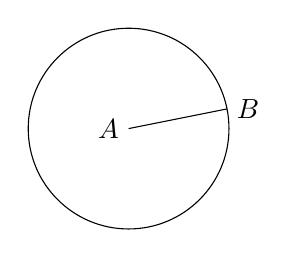
\begin{tikzpicture}
  \coordinate [label=left:$A$]  (A) at (0,0);
  \coordinate [label=right:$B$] (B) at (1.25,0.25);
  \draw (A) -- (B);

  \draw (A) let
              \p1 = ($ (B) - (A) $)
            in
              circle ({veclen(\x1,\y1)});
\end{tikzpicture}
\end{codeexample}

\bohs

% Each assignment in a let operation starts with |\p|, usually followed
% by a \meta{digit}. Then comes an equal sign and a coordinate. The
% coordinate is evaluated and the result is stored internally. From
% then on you can use the following expressions: 
\ltz{let} 操作的每一次赋值都从 \ltz{\\p} 开始,通常跟着一个~{\color{blue}\metazh{数字}},接着是一个等号和一个坐标。
计算好坐标后,结果保存在内部,之后你就可以用下面的表达式:

\eohs

\begin{enumerate}
% \item |\x|\meta{digit} yields the $x$-coordinate of the resulting point.
\item \ltz{\\x}{\color{blue}\metazh{数字}} 得到对应点的 $x$ 坐标。
% \item |\y|\meta{digit} yields the $y$-coordinate of the resulting point.
\item \ltz{\\y}{\color{blue}\metazh{数字}} 得到对应点的 $y$ 坐标。
% \item |\p|\meta{digit} yields the same as |\x|\meta{digit}|,\y|\meta{digit}.
\item \ltz{\\p}{\color{blue}\metazh{数字}} 等同于 \ltz{\\x}{\color{blue}\metazh{数字}}\ltz{,\\y}{\color{blue}\metazh{数字}}。
\end{enumerate}

\bohs

% You can have multiple assignments in a let operation, just separate
% them with commas. In later assignments you can already use the results
% of earlier assignments.
你可以在 \ltz{let} 操作中赋很多值,只要用逗号隔开。
后面的赋值可以使用前面的赋值结果。

% Note that |\p1| is not a coordinate in the usual sense. Rather, it
% just expands to a string like |10pt,20pt|. So, you cannot write, for
% instance, |(\p1.center)| since this would just expand to
% |(10pt,20pt.center)|, which makes no sense.
注意,\ltz{\\p1} 并不是通常意义上的坐标,它只是扩展成 \ltz{10pt,20pt} 这样的字符串。
因此,你不能写 \ltz{(\\p1.center)} 这样的语句,因为这个只会扩展成 \ltz{(10pt,20pt.center)},这条语句没有意义。

% Next, we want to draw both circles at the same time. Each time the
% radius is |veclen(\x1,\y1)|. It seems natural to compute this radius
% only once. For this, we can also use a let operation: Instead of
% writing |\p1 = ...|, we write |\n2 = ...|. Here, ``n'' stands for
% ``number'' (while ``p'' stands for ``point''). The assignment of a
% number should be followed by a number in curly braces.
下一步,我们想同时将两个圆画出来。
两个圆半径都是 \ltz{veclen(\\x1,\\y1)},因此自然只需要计算一次。
这里我们还可以用一个 \ltz{let} 操作:不是写 \ltz{\\p1 = ...},而是写 \ltz{\\n2 = ...}。
这里的 \ltz{n} 表示 “数”(\textbf{n}umber),同理,\ltz{p} 表示“点”(\textbf{p}oint)。
给数赋值需要在外面加上花括号。

\eohs

\begin{codeexample}[]
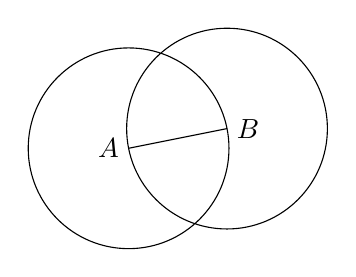
\begin{tikzpicture}
  \coordinate [label=left:$A$]  (A) at (0,0);
  \coordinate [label=right:$B$] (B) at (1.25,0.25);
  \draw (A) -- (B);

  \draw let \p1 = ($ (B) - (A) $),
            \n2 = {veclen(\x1,\y1)}
        in
          (A) circle (\n2)
          (B) circle (\n2);
\end{tikzpicture}
\end{codeexample}

\bohs

% In the above example, you may wonder, what |\n1| would yield? The
% answer is that it would be undefined -- the |\p|, |\x|, and |\y|
% macros refer to the same logical point, while the |\n| macro has ``its
% own namespace.'' We could even have replaced |\n2| in the example by
% |\n1| and it would still work. Indeed, the digits following these
% macros are just normal \TeX\ parameters. We could also use a longer
% name, but then we have to use curly braces:
看了上例,你可能会想,如果写 \ltz{\\n1} 会得到什么?
答案是会显示它没有定义。
宏 \ltz{\\p}、\ltz{\\x} 和 \ltz{\\y} 引用逻辑上的同一个点,而宏 \ltz{\\n} 则有“自己的命名空间”。
我们甚至可以将例中的 \ltz{\\n2} 替换成 \ltz{\\n1},效果一样。
事实上,跟在这些宏后面的数字只是普通的 \TeX\ 参数。
我们还可以用更长的名字,不过需要加上花括号:

\eohs

\begin{codeexample}[]
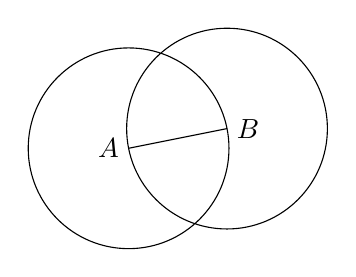
\begin{tikzpicture}
  \coordinate [label=left:$A$]  (A) at (0,0);
  \coordinate [label=right:$B$] (B) at (1.25,0.25);
  \draw (A) -- (B);

  \draw let \p1        = ($ (B) - (A) $),
            \n{radius} = {veclen(\x1,\y1)}
        in
          (A) circle (\n{radius})
          (B) circle (\n{radius});
\end{tikzpicture}
\end{codeexample}

\bohs

% At the beginning of this section it was promised that there is an
% easier way to create the desired circle. The trick is to use the
% |through| library. As the name suggests, it contains code for creating
% shapes that go through a given point.
在本节开始我们答应过,有个更简单的方法画出想要的圆。
这个技巧就是用 \ltz{through} 库。
顾名思义,它的作用就是通过一个给定的点创建形状。

% The option that we are looking for is |circle through|. This option is
% given to a \emph{node} and has the following effects: First, it causes
% the node's inner and outer separations to be set to zero. Then it sets
% the shape of the node to |circle|. Finally, it sets the radius of the
% node such that it goes through the parameter given to
% |circle through|. This radius is computed in essentially the same way
% as above.
我们要找的选项是 \ltz{circle through}。
这个选项传给一个\emph{节点},产生如下效果:
首先,它将节点的内外间距置零;然后,将节点的形状设为圆 \ltz{circle};最后,它根据传给 \ltz{circle through} 的参数决定圆的半径,本质上,计算该半径的方法和上面一样。

\eohs

\begin{codeexample}[]
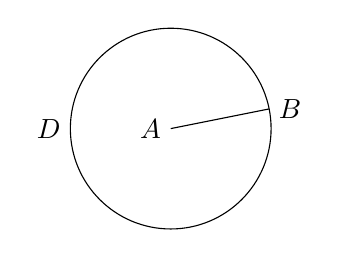
\begin{tikzpicture}
  \coordinate [label=left:$A$]  (A) at (0,0);
  \coordinate [label=right:$B$] (B) at (1.25,0.25);
  \draw (A) -- (B);

  \node [draw,circle through=(B),label=left:$D$] at (A) {};
\end{tikzpicture}
\end{codeexample}


% \subsubsection{The Intersection of the Circles}
\subsubsection{圆的交点}

\bohs

% Euclid can now draw the line and the circles. The final problem is to
% compute the intersection of the two circles. This computation is a bit
% involved if you want to do it ``by hand.'' Fortunately, the
% intersection library allows us to compute the intersection of
% arbitrary paths.
Euclid 现在可以画线和圆了。
最后一个问题就是计算两圆的交点,这就涉及到你是否想“手算”它。
好在 \ltz{intersections} 库可以让我们计算任意路径的交点。

% The idea is simple: First, you ``name'' two paths using the
% |name path| option. Then, at some later point, you can use the option
% |name intersections|, which creates coordinates called
% |intersection-1|, |intersection-2|, and so on at all intersections of
% the paths. Euclid assigns the names |D| and |E| to the paths of the
% two circles (which happen to be the same names as the nodes
% themselves, but nodes and their paths live in different
% ``namespaces''). 
思路很简单:首先用 \ltz{name path} 选项“命名”两条路径;接着,你可以在之后用 \ltz{name intersections} 选项,这会在路径之间的所有交点处创建坐标,名为 \ltz{intersection-1}、\ltz{intersection-2} 等等。
Euclid 将两圆交点命名为 \ltz{D} 和 \ltz{E}(恰好和节点重名,不过节点和路径拥有不同的“命名空间”)。

\eohs

\begin{codeexample}[]
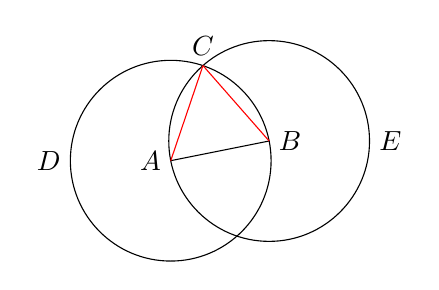
\begin{tikzpicture}
  \coordinate [label=left:$A$]  (A) at (0,0);
  \coordinate [label=right:$B$] (B) at (1.25,0.25);
  \draw (A) -- (B);

  \node (D) [name path=D,draw,circle through=(B),label=left:$D$]  at (A) {};
  \node (E) [name path=E,draw,circle through=(A),label=right:$E$] at (B) {};

  % 给坐标命名,但是什么都不画:
  \path [name intersections={of=D and E}];
  
  \coordinate [label=above:$C$] (C) at (intersection-1);

  \draw [red] (A) -- (C);
  \draw [red] (B) -- (C);
\end{tikzpicture}
\end{codeexample}

\bohs

% It turns out that this can be further shortened: The
% |name intersections| takes an optional argument |by|, which lets you
% specify names for the coordinates and options for them. This creates
% more compact code. Although Euclid does not need it for the current
% picture, it is just a small step to computing the bisection of the line $AB$:
这可以进一步简写:
\ltz{name intersections} 有一个可选参数 \ltz{by},你可以用它指定坐标的名称和选项,这让代码更紧凑。
虽然 Euclid 画现在这张图还用不到,但是画线段 $AB$ 的平分线时,用这个参数只需要一小步。

\eohs

\begin{codeexample}[]
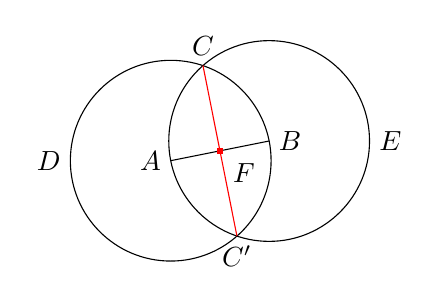
\begin{tikzpicture}
  \coordinate [label=left:$A$]  (A) at (0,0);
  \coordinate [label=right:$B$] (B) at (1.25,0.25);
  \draw [name path=A--B] (A) -- (B);

  \node (D) [name path=D,draw,circle through=(B),label=left:$D$]  at (A) {};
  \node (E) [name path=E,draw,circle through=(A),label=right:$E$] at (B) {};

  \path [name intersections={of=D and E, by={[label=above:$C$]C, [label=below:$C'$]C'}}];

  \draw [name path=C--C',red] (C) -- (C');

  \path [name intersections={of=A--B and C--C',by=F}];
  \node [fill=red,inner sep=1pt,label=-45:$F$] at (F) {};
\end{tikzpicture}
\end{codeexample}

% \subsubsection{The Complete Code}
\subsubsection{完整代码}

\bohs

% Back to Euclid's code. He introduces a few macros to make life
% simpler, like a |\A| macro for typesetting a blue $A$. He also uses the
% |background| layer for drawing the triangle behind everything at the
% end. 
回到 Euclid 的代码,人生苦短,他写了几个宏。比如用 \ltz{\\A} 表示一个蓝色的 $A$,他还用了 \ltz{background} 层,在结尾处画了一个三角形,并置于最底层。

\eohs

\begin{codeexample}[]
\begin{tikzpicture}[thick,help lines/.style={thin,draw=black!50}]
  \def\A{\textcolor{input}{$A$}}     \def\B{\textcolor{input}{$B$}}
  \def\C{\textcolor{output}{$C$}}    \def\D{$D$}
  \def\E{$E$}
  
  \colorlet{input}{blue!80!black}    \colorlet{output}{red!70!black}
  \colorlet{triangle}{orange}
  
  \coordinate [label=left:\A]  (A) at ($ (0,0) + .1*(rand,rand) $);
  \coordinate [label=right:\B] (B) at ($ (1.25,0.25) + .1*(rand,rand) $);

  \draw [input] (A) -- (B);
  
  \node [name path=D,help lines,draw,label=left:\D]   (D) at (A) [circle through=(B)] {};
  \node [name path=E,help lines,draw,label=right:\E]  (E) at (B) [circle through=(A)] {};
  
  \path [name intersections={of=D and E,by={[label=above:\C]C}}];

  \draw [output] (A) -- (C) -- (B);

  \foreach \point in {A,B,C}
    \fill [black,opacity=.5] (\point) circle (2pt);

  \begin{pgfonlayer}{background}
    \fill[triangle!80] (A) -- (C) -- (B) -- cycle;
  \end{pgfonlayer}
  
  \node [below right, text width=10cm,align=justify] at (4,3) {
    \small
    \textbf{命题 1}\par
    \emph{在一条已知\textcolor{input}{有限直线}上作一个\textcolor{triangle}{等边三角形}.}
    \par\vskip1em
    设 \A\B\ 是已知\textcolor{input}{有限直线}. \dots
  };
\end{tikzpicture}
\end{codeexample}

\clearpage
% \subsection{Book I, Proposition II}
\subsection{卷 I,命题 2}

\bohs

% The second proposition in the Elements is the following:
《几何原本》中的第二个命题如下:

\eohs

\bigskip\noindent
\begin{tikzpicture}[thick,help lines/.style={thin,draw=black!50}]
  \def\A{\textcolor{orange}{$A$}}   \def\B{\textcolor{input}{$B$}}
  \def\C{\textcolor{input}{$C$}}    \def\D{$D$}
  \def\E{$E$}                       \def\F{$F$}
  \def\G{$G$}                       \def\H{$H$}
  \def\K{$K$}                       \def\L{\textcolor{output}{$L$}}
  
  \colorlet{input}{blue!80!black}    \colorlet{output}{red!70!black}
  
  \coordinate [label=left:\A]  (A) at ($ (0,0) + .1*(rand,rand) $);
  \coordinate [label=right:\B] (B) at ($ (1,0.2) + .1*(rand,rand) $);
  \coordinate [label=above:\C] (C) at ($ (1,2) + .1*(rand,rand) $);

  \draw [input] (B) -- (C);
  \draw [help lines] (A) -- (B);

  \coordinate [label=above:\D] (D) at ($ (A)!.5!(B) ! {sin(60)*2} ! 90:(B) $);

  \draw [help lines] (D) -- ($ (D)!3.75!(A) $) coordinate [label=-135:\E] (E);
  \draw [help lines] (D) -- ($ (D)!3.75!(B) $) coordinate [label=-45:\F] (F);

  \node (H) at (B) [name path=H,help lines,circle through=(C),draw,label=135:\H] {};
  \path [name path=B--F] (B) -- (F);
  \path [name intersections={of=H and B--F}]
    coordinate [label=right:\G] (G) at (intersection-1);

  \node (K) at (D) [name path=K,help lines,circle through=(G),draw,label=135:\K] {};

  \path [name path=A to E line] (A) -- (E);
  \path [name intersections={of=K and A to E line}]
    coordinate [label=below:\L] (L) at (intersection-1);

  \draw [output] (A) -- (L);

  \foreach \point in {A,B,C,D,G,L}
    \fill [black,opacity=.5] (\point) circle (2pt);
  
  \node [below right, text width=9cm,align=justify] at (4,4) {
    \small
    % \textbf{Proposition II}\par
    \textbf{命题 2} \par
    % \emph{To place a \textcolor{output}{straight line} equal to a
    %   given \textcolor{input}{straight line} with 
    %   one end at a \textcolor{orange}{given point}.} 
    \emph{以一个\textcolor{orange}{已知点}作为端点,作一条\textcolor{output}{线段}与已知\textcolor{input}{线段}相等.}
    \par\vskip1em
    % Let \A\ be the given point, and \B\C\ the given
    % \textcolor{input}{straight line}. 
    % It is required to place a \textcolor{output}{straight line} equal
    % to the given \textcolor{input}{straight line} \B\C\ with one end
    % at the point~\A.  
    设 \A\ 为已知点,\B\C\ 为已知\textcolor{input}{线段}.
    要求以 \A\ 为端点,作一条\textcolor{output}{线段}与已知\textcolor{input}{线段} \B\C\ 相等.

    % Join the straight line \A\B\ from the point \A\ to the point \B, and
    % construct the equilateral triangle \D\A\B\ on it.
    连接点 \A\ 和 \B\ 得线段 \A\B ,并在其上作一等边三角形 \D\A\B .
    
    % Produce the straight lines \A\E\ and \B\F\ in a straight line with
    % \D\A\ and \D\B. Describe the circle \C\G\H\ with center \B\ and
    % radius \B\C, and  again, describe the circle \G\K\L\ with center
    % \D\ and radius \D\G. 	
    延长 \D\A\ 和 \D\B\ 为直线 \A\E\ 和 \B\F 。以 \B\ 为中心,\B\C\ 为半径,作圆 \C\G\H ,再以 \D\ 为中心,\D\G\ 为半径,作圆 \G\K\L .

    % Since the point \B\ is the center of the circle \C\G\H, therefore
    % \B\C\ equals \B\G. Again, since the point \D\ is the center of the
    % circle \G\K\L, therefore \D\L\ equals \D\G. And in these \D\A\
    % equals \D\B, therefore the remainder \A\L\ equals the remainder
    % \B\G. But \B\C\ was also proved  equal to \B\G, therefore each of
    % the straight lines \A\L\ and \B\C\ equals \B\G. And things which
    % equal the same thing also equal one another, therefore \A\L\ also
    % equals \B\C. 
    因为点 \B\ 是圆 \C\G\H\ 的圆心,所以 \B\C\ 等于 \B\G .
    同样,因为点 \D\ 是圆 \G\K\L\ 的圆心,所以 \D\L\ 等于 \D\G .
    又因为 \D\A\ 等于 \D\B ,因此线段之差 \A\L\ 等于线段之差 \B\G .
    然而已经证明了 \B\C\ 等于 \B\G ,所以 \A\L\ 和 \B\C\ 均等于 \B\G .
    而且等于同量的量彼此相等,所以 \A\L\ 也等于 \B\C .

    % Therefore the \textcolor{output}{straight line} \A\L\ equal to the
    % given \textcolor{input}{straight line} \B\C\  has been placed with
    % one end at the \textcolor{orange}{given point}~\A.  
    所以,由已知点 \A\ 作出了\textcolor{output}{线段} \A\L\ ,与已知\textcolor{input}{线段} \B\C\ 相等.
  };
\end{tikzpicture}


% \subsubsection{Using Partway Calculations for the Construction of \emph{D}}
\subsubsection{用分比计算构造点 \emph{D}}

\bohs

% Euclid's construction starts with ``referencing'' Proposition~I for
% the construction of the point~$D$. Now, while we could simply repeat the
% construction, it seems a bit bothersome that one has to draw all these
% circles and do all these complicated constructions.
Euclid 在构造点 $D$ 时,“参考”了命题 1 中的过程。
现在,我们也可以简单重复这些构造过程,但是似乎有点麻烦,因为我们得画出所有这些圆,完成所有复杂的构造。

% For this reason, \tikzname\ supports some simplifications. First,
% there is a simple syntax for computing a point that is ``partway'' on
% a line from $p$ to~$q$: You place these two points in a coordinate
% calculation -- remember, they start with |($| and end with |$)| -- and
% then combine them using |!|\meta{part}|!|. A \meta{part} of |0| refers
% to the \emph{first} coordinate, a \meta{part} of |1| refers to the
% second coordinate, and a value in between refers to a point on the
% line from $p$ to~$q$. Thus, the syntax is similar to the |xcolor|
% syntax for mixing colors.
因此,\tikzname\ 提供了简便方法。
首先,有一个简单的语法,可以计算从 $p$ 到 $q$ 连线上的一点:
将这两个点放到坐标计算环境中——别忘了首尾的 \ltz{($} 和 \ltz{$)}——
然后用 \ltz{!}\metablue{分比}\ltz{!} 将它们组合起来。
\metablue{分比} 为 \ltz{0} 表示 \emph{前面的}坐标,\metablue{分比} 为 \ltz{1} 表示\emph{后面的}坐标,\ltz{0} 到 \ltz{1} 之间的值表示两点连线上的一点。
所以,这个语法类似于 \ltz{xcolor} 中混合颜色的语法。

% Here is the computation of the point in the middle of the line $AB$:
这里展示了如何计算线段 $AB$ 的中点:

\eohs

\begin{codeexample}[]
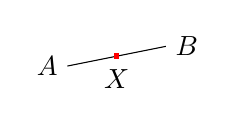
\begin{tikzpicture}
  \coordinate [label=left:$A$]  (A) at (0,0);
  \coordinate [label=right:$B$] (B) at (1.25,0.25);
  \draw (A) -- (B);
  \node [fill=red,inner sep=1pt,label=below:$X$] (X) at ($ (A)!.5!(B) $) {};
\end{tikzpicture}
\end{codeexample}

\bohs

% The computation of the point $D$ in Euclid's second proposition is a
% bit more complicated. It can be expressed as follows: Consider the
% line from $X$ to $B$. Suppose we 
% rotate this line around $X$ for 90$^\circ$ and then stretch it by a
% factor of $\sin(60^\circ) \cdot 2$. This yields the desired point~$D$. We
% can do the stretching using the partway modifier above, for the
% rotation we need a new modifier: the rotation modifier. The idea is
% that the second coordinate in a partway computation can be prefixed by
% an angle. Then the partway point is computed normally (as if no angle
% were given), but the resulting point is rotated by this angle around
% the first point. 
在 Euclid 的命题 2 中,点 D 的计算更加复杂。
可以表述如下:考虑 $X$ 到 $B$ 的直线,假设我们将该直线以 $X$ 为中心,旋转 90$^\circ$,然后拉伸 $\sin(60^\circ \cdot 2$ 倍,得到点 $D$。
我们可以用上面的分比调节器实现拉伸,然后用另外一个调节器实现旋转。
思路是,在分比计算中,可以在第二个坐标前加上一个角度,接着会正常计算分比得到的点(就像没加角度参数一样),然后再将该点以第一个坐标为心旋转给定的角度。

\eohs

\begin{codeexample}[]
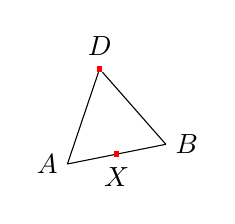
\begin{tikzpicture}
  \coordinate [label=left:$A$]  (A) at (0,0);
  \coordinate [label=right:$B$] (B) at (1.25,0.25);
  \draw (A) -- (B);
  \node [fill=red,inner sep=1pt,label=below:$X$] (X) at ($ (A)!.5!(B) $) {};
  \node [fill=red,inner sep=1pt,label=above:$D$] (D) at
    ($ (X) ! {sin(60)*2} ! 90:(B) $) {};
  \draw (A) -- (D) -- (B);
\end{tikzpicture}
\end{codeexample}

\bohs

% Finally, it is not necessary to explicitly name the point $X$. Rather,
% again like in the |xcolor| package, it is possible to chain partway
% modifiers:
最后,其实不必显式地将点命名为 $X$,而是可以像 \ltz{xcolor} 宏包那样,使用链式语法。

\eohs

\begin{codeexample}[]
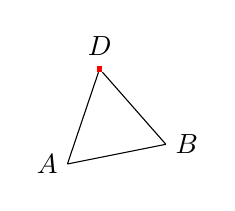
\begin{tikzpicture}
  \coordinate [label=left:$A$]  (A) at (0,0);
  \coordinate [label=right:$B$] (B) at (1.25,0.25);
  \draw (A) -- (B);
  \node [fill=red,inner sep=1pt,label=above:$D$] (D) at
    ($ (A) ! .5 ! (B) ! {sin(60)*2} ! 90:(B) $) {};
  \draw (A) -- (D) -- (B);
\end{tikzpicture}
\end{codeexample}


% \subsubsection{Intersecting a Line and a Circle}
\subsubsection{直线和圆相交}

\bohs

% The next step in the construction is to draw a circle around $B$
% through $C$, which is easy enough to do using the |circle through|
% option. Extending the lines $DA$ and $DB$ can be done using partway
% calculations, but this time with a part value outside the range
% $[0,1]$: 
下一步构造是以 $B$ 为圆心,过 $C$ 画一个圆,用 \ltz{circle through} 很容易实现。
延长 $DA$ 和 $DB$ 则可以用分比计算,只不过这次的分比在范围 $[0,1]$ 外:

\eohs

\begin{codeexample}[]
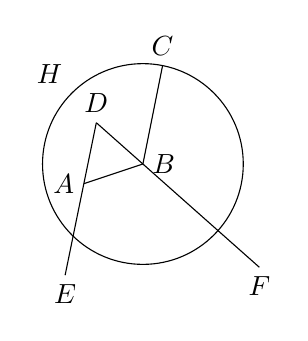
\begin{tikzpicture}
  \coordinate [label=left:$A$]  (A) at (0,0);
  \coordinate [label=right:$B$] (B) at (0.75,0.25);
  \coordinate [label=above:$C$] (C) at (1,1.5);
  \draw (A) -- (B) -- (C);
  \coordinate [label=above:$D$] (D) at
    ($ (A) ! .5 ! (B) ! {sin(60)*2} ! 90:(B) $) {};
  \node (H) [label=135:$H$,draw,circle through=(C)] at (B) {};
  \draw (D) -- ($ (D) ! 3.5 ! (B) $) coordinate [label=below:$F$] (F);
  \draw (D) -- ($ (D) ! 2.5 ! (A) $) coordinate [label=below:$E$] (E);
\end{tikzpicture}
\end{codeexample}

\bohs

% We now face the problem of finding the point $G$, which is the
% intersection of the line $BF$ and the circle $H$. One way is to use
% yet another variant of the partway computation: Normally, a partway
% computation has the form \meta{p}|!|\meta{factor}|!|\meta{q},
% resulting in the point $(1-\meta{factor})\meta{p} +
% \meta{factor}\meta{q}$. Alternatively, instead of \meta{factor} you
% can also use a \meta{dimension} between the points. In this case, you
% get the point that is \meta{dimension} away from \meta{p} on the
% straight line to \meta{q}.
我们现在的问题是如何得到点 $G$,也就是线 $BF$ 和圆 $H$ 的交点。
一个方法是对分比计算进行变形:
正常的分比计算形式是 \metablue{p}\ltz{!}\metablue{分比}\ltz{!}\metablue{q},得到点~{\color{blue} (1 - \metazh{分比}) \meta{p} + \metazh{分比} \meta{q}}。
除了 \metablue{分比}(factor),在两点之间你还可以用 \metablue{长度}(dimension),\footnote{{\color{blue} 关于“分比”一词的原文,作者前面用的是 part,这里用了 factor,为了一致,这里统一译为“分比”。}} \footnote{{\color{blue} dimension 直译应为“维度”、“量纲”或者“尺寸”,但是这里为了更贴合其实际含义,译成了“长度”。}}
这时你得到的点,则在 \metablue{p} 到 \metablue{q} 的直线上,并且到 \metablue{q} 的距离为 \metablue{长度}。


% We know that the point $G$ is on the way from $B$ to $F$. The distance
% is given by the radius of the circle~$H$. Here is the code for
% computing $H$:
我们知道点 $G$ 在 $B$ 到 $F$ 的直线上,$G$ 到 $B$ 的距离等于圆 $H$ 的半径。
计算 $H$ 的代码如下:

\eohs

{\tikzexternaldisable
\begin{codeexample}[pre={
\begin{tikzpicture}
  \coordinate [label=left:$A$]  (A) at (0,0);
  \coordinate [label=right:$B$] (B) at (0.75,0.25);
  \coordinate [label=above:$C$] (C) at (1,1.5);
  \draw (A) -- (B) -- (C);
  \coordinate [label=above:$D$] (D) at
    ($ (A) ! .5 ! (B) ! {sin(60)*2} ! 90:(B) $) {};
  \draw (D) -- ($ (D) ! 3.5 ! (B) $) coordinate [label=below:$F$] (F);
  \draw (D) -- ($ (D) ! 2.5 ! (A) $) coordinate [label=below:$E$] (E);
},post={\end{tikzpicture}}]
  \node (H) [label=135:$H$,draw,circle through=(C)] at (B) {};
  \path let \p1 = ($ (B) - (C) $) in
    coordinate [label=left:$G$] (G) at ($ (B) ! veclen(\x1,\y1) ! (F) $);
  \fill[red,opacity=.5] (G) circle (2pt);
\end{codeexample}

\bohs

% However, there is a simpler way: We can simply name the path of the
% circle and of the line in question and then use |name intersections|
% to compute the intersections.
不过有个更简单的方法:
我们只要给题中圆和线的路径命名,然后用 \ltz{name intersection} 来计算交点。

\eohs

\begin{codeexample}[pre={
\begin{tikzpicture}
  \coordinate [label=left:$A$]  (A) at (0,0);
  \coordinate [label=right:$B$] (B) at (0.75,0.25);
  \coordinate [label=above:$C$] (C) at (1,1.5);
  \draw (A) -- (B) -- (C);
  \coordinate [label=above:$D$] (D) at
    ($ (A) ! .5 ! (B) ! {sin(60)*2} ! 90:(B) $) {};
  \draw (D) -- ($ (D) ! 3.5 ! (B) $) coordinate [label=below:$F$] (F);
  \draw (D) -- ($ (D) ! 2.5 ! (A) $) coordinate [label=below:$E$] (E);
},post={\end{tikzpicture}}]
  \node (H) [name path=H,label=135:$H$,draw,circle through=(C)] at (B) {};
  \path [name path=B--F] (B) -- (F);
  \path [name intersections={of=H and B--F,by={[label=left:$G$]G}}];
  \fill[red,opacity=.5] (G) circle (2pt);
\end{codeexample}
}%

% \subsubsection{The Complete Code}
\subsubsection{完整代码}

\begin{codeexample}[]
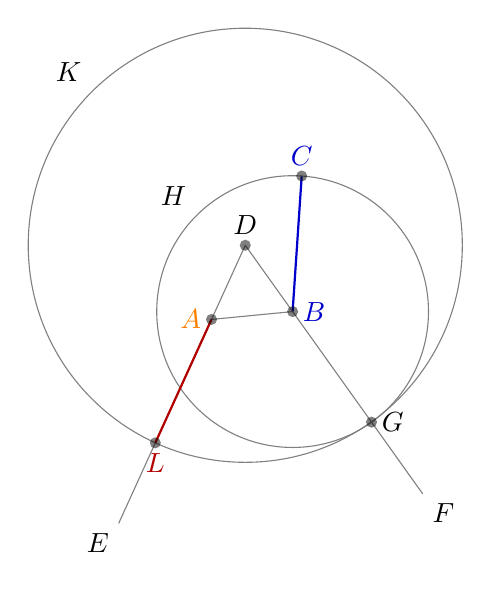
\begin{tikzpicture}[thick,help lines/.style={thin,draw=black!50}]
  \def\A{\textcolor{orange}{$A$}}   \def\B{\textcolor{input}{$B$}}
  \def\C{\textcolor{input}{$C$}}    \def\D{$D$}
  \def\E{$E$}                       \def\F{$F$}
  \def\G{$G$}                       \def\H{$H$}
  \def\K{$K$}                       \def\L{\textcolor{output}{$L$}}
  
  \colorlet{input}{blue!80!black}    \colorlet{output}{red!70!black}
  
  \coordinate [label=left:\A]  (A) at ($ (0,0) + .1*(rand,rand) $);
  \coordinate [label=right:\B] (B) at ($ (1,0.2) + .1*(rand,rand) $);
  \coordinate [label=above:\C] (C) at ($ (1,2) + .1*(rand,rand) $);

  \draw [input] (B) -- (C);
  \draw [help lines] (A) -- (B);

  \coordinate [label=above:\D] (D) at ($ (A)!.5!(B) ! {sin(60)*2} ! 90:(B) $);

  \draw [help lines] (D) -- ($ (D)!3.75!(A) $) coordinate [label=-135:\E] (E);
  \draw [help lines] (D) -- ($ (D)!3.75!(B) $) coordinate [label=-45:\F] (F);

  \node (H) at (B) [name path=H,help lines,circle through=(C),draw,label=135:\H] {};
  \path [name path=B--F] (B) -- (F);
  \path [name intersections={of=H and B--F,by={[label=right:\G]G}}];

  \node (K) at (D) [name path=K,help lines,circle through=(G),draw,label=135:\K] {};
  \path [name path=A--E] (A) -- (E);
  \path [name intersections={of=K and A--E,by={[label=below:\L]L}}];

  \draw [output] (A) -- (L);

  \foreach \point in {A,B,C,D,G,L}
    \fill [black,opacity=.5] (\point) circle (2pt);

  % \node ...
\end{tikzpicture}
\end{codeexample}
